% Chapter X

\chapter{Modelos de Web Caché} % Chapter title

\label{ch:modelos_web_caching} % For referencing the chapter elsewhere, use \autoref{ch:name} 

El web caché no es un concepto nuevo. Este tema ya se ha estudiado y también ha sido objeto de numerosos papers, artículos y tesis. Por otro lado el concepto de caché web distribuida es un poco más nuevo pero también suma bastantes proyectos entorno a él.

Como primer acercamiento, es necesario definir el el significado de caché web (en ocasiones también llamado proxy) \cite{wiki_cacheweb}:

"Se llama caché web a la caché que almacena documentos web (es decir, páginas, imágenes, entre otros) para reducir el ancho de banda consumido, la carga de los servidores y el retardo en la descarga. Un caché web almacena copias de los documentos que pasan por él, de forma que subsiguientes peticiones pueden ser respondidas por el propio caché, si se cumplen ciertas condiciones." 

En resumen, se podría entender una caché web como una forma de almacenar temporalmente documentos que son concurrentemente solicitado con el fin de reducir el ancho de banda saliente. Por otro lado, la presente investigación se centra en modelos que comparten dinámicamente éstos documentos. 

Un concepto muy parecido es el de caché web cooperativo. Según Rowstron A. \cite{rowstron:2001} mediante esta técnica, el almacenamiento dedicado a la caché de una serie de servidores-proxy adyacentes se gestiona conjuntamente como si se tratase de una única cache distribuida. Las políticas de gestión de esta cache se realiza teniendo en cuenta el estado y los contenidos de todos los servidores-proxy que la componen. Por ejemplo, las políticas de reemplazo en la cache cooperativa tendrán en cuenta las estadísticas de acceso en todos los servidores-proxy cooperantes.

El caché web cooperativo permite incrementar considerablemente el tamaño de la caché, pero a costa de
reducir la probabilidad de acierto local. Bajo éste esquema, un único servidor-proxy no dispone de los contenidos más populares, provocando un aumento del porcentaje de peticiones que se tienen que servir remotamente desde los otros servidores que componen la cache ó desde el servidor principal.

Basado en la investigación del estado del arte, se han podido identificar proyectos que giran alrededor de la presente tesis. Entre ellos están: CoralCDN \cite{freedman:2004}, Transparent Distributed Web Caching \cite{liang:2001}, Dalesa \cite{wathsala:2009} y Squirrel \cite{rowstron:2001}.


%----------------------------------------------------------------------------------------

\section{Web Caching mediante Proxy}

%------------------------------------------------

\subsection{Proxy Simple}

Primero se mostrará el modelo tradicional de cliente-servidor. Bajo este modelo el cliente tiene una conexión directa con el servidor y no existe caché en medio, por lo que en dicha conexión se obtienen los servicios bajo demanda, haciendo uso únicamente del caché local del explorador web.

\begin{figure}[h]
  \centering
    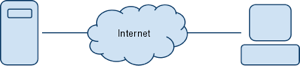
\includegraphics[scale=1]{gfx/proxy_simple_1}
  \caption{Conexión Directa}
  \label{proxy_simple_1}		
\end{figure}

La siguiente figura \ref{proxy_simple_2} muestra el típico modelo de proxy, donde existe un servidor central por el cual los clientes transitan y le solicitan el recurso deseado. El servidor proxy descarga el recurso solicitado, lo almacena en su caché y por último lo reenvía al solicitante. Si otro cliente solicitara el mismo recurso, el servidor le respondería con el recurso almacenado localmente (si la caché haya caducado aún).

\begin{figure}[h]
  \centering
    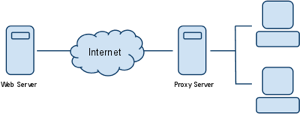
\includegraphics[scale=1]{gfx/proxy_simple_2}
  \caption{Proxy Simple}
  \label{proxy_simple_2}
\end{figure}

%------------------------------------------------

\subsection{Proxy Jerárquico}

La figura \ref{proxy_jerarquico} muestra el modelo de proxy jerárquico o también conocido como web caché cooperativo. En este modelo se tienen servidores proxy ubicados de una manera jerárquica en una Red de área local. Cuando un cliente solicita un recurso, éste lo hace a su proxy jerárquicamente más cercano. Si dicho servidor posee los recursos éste se lo reenvía al cliente. En caso que no posee el recurso, el proxy le reenvía la solicitud de su cliente al servidor proxy de nivel superior. Si el servidor de nivel superior posee el recurso lo reenvía al servidor proxy que solicitó el recurso, éste último se deja una copia en su caché local y reenvía el recurso al cliente original.

\begin{figure}[h]
  \centering
    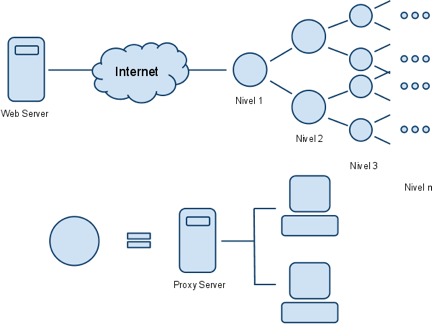
\includegraphics[scale=0.75]{gfx/proxy_jerarquico}
  \caption{Proxy Jerárquico}
  \label{proxy_jerarquico}
\end{figure}

%----------------------------------------------------------------------------------------

\subsection{Proxy Descentralizado}

Bajo este modelo se encuentran los proyectos de Squirrel y Dalesa. Estos proyectos intentan utilizar los conceptos de P2P para implementar y compartir una cache distribuida a través de una LAN. Como se muestra en la figura \ref{proxy_descentralizado}. Cada computadora forma parte del proxy descentralizado, y utilizando un software creado por los respectivos participantes del proyecto, pueden compartir la cache. Este modelo es el que más se acerca al modelo que se propone como tesis aunque todavía dista en ciertas características.

\begin{figure}[h]
  \centering
    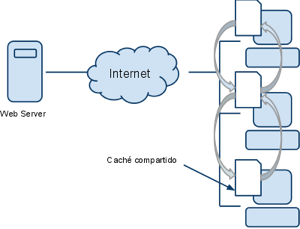
\includegraphics[scale=1]{gfx/proxy_descentralizado}
  \caption{Proxy Descentralizado}
  \label{proxy_descentralizado}
\end{figure}

\section{Redes CDN}
Una red de distribución de contenidos es una red de equipos que opera de forma transparente para entregar contenido de sus clientes cumpliendo principalmente alguno de los siguientes objetivos:
\begin{enumerate}
\item Escalabilidad
\item Coste
\item Eficiencia
\end{enumerate}

Haciendo una definición más amplia una Red CDN es un sistema de computadoras el cual contiene copias de datos, ubicados en varios puntos de la red para así maximizar el ancho de banda para el acceso de los datos desde los clientes a través de la red. Un cliente accede una copia de los datos, la más cercana, contrario al concepto de que todos los clientes accedan al mismo servidor central provocando un cuello de botella en el servidor \cite{wiki_cdn}.

El contenido puede incluir objetos web, objetos descargables (archivos de medios, software, documentos, entre otros), aplicaciones, media streams en tiempo real, y otros componentes.

En la siguiente figura se puede observar el funcionamiento de una Red CDN distribuida a través de Internet.

\begin{figure}[h]
  \centering
    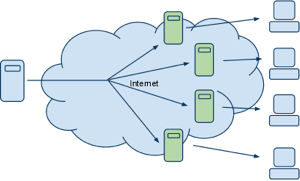
\includegraphics[scale=1]{gfx/redes_cdn}
  \caption{Red CDN}
  \label{conexionhttp}
\end{figure}
